%%%%%%%%%%%%%%%%%%%%%%%%%%%%%%%%%%%%%%%%%%%%%%%%%%%%%%%%%%%%%%%%%%%%%%
% LaTeX Example: Project Report
%
% Source: http://www.howtotex.com
%
% Feel free to distribute this example, but please keep the referral
% to howtotex.com
% Date: March 2011 
% 
%%%%%%%%%%%%%%%%%%%%%%%%%%%%%%%%%%%%%%%%%%%%%%%%%%%%%%%%%%%%%%%%%%%%%%
% How to use writeLaTeX: 
%
% You edit the source code here on the left, and the preview on the
% right shows you the result within a few seconds.
%
% Bookmark this page and share the URL with your co-authors. They can
% edit at the same time!
%
% You can upload figures, bibliographies, custom classes and
% styles using the files menu.
%
% If you're new to LaTeX, the wikibook is a great place to start:
% http://en.wikibooks.org/wiki/LaTeX
%
%%%%%%%%%%%%%%%%%%%%%%%%%%%%%%%%%%%%%%%%%%%%%%%%%%%%%%%%%%%%%%%%%%%%%%
% Edit the title below to update the display in My Documents
%\title{Project Report}
%
%%% Preamble
\documentclass[paper=a4, fontsize=11pt]{scrartcl}
\usepackage[T1]{fontenc}
\usepackage{fourier}

\usepackage[english]{babel}                                                         % English language/hyphenation
\usepackage[protrusion=true,expansion=true]{microtype}  
\usepackage{amsmath,amsfonts,amsthm} % Math packages
\usepackage[pdftex]{graphicx}   
\usepackage{epstopdf}
\epstopdfsetup{outdir=./}
\usepackage{url}
\usepackage{subfigure}


%%% Custom sectioning
\usepackage{sectsty}
\allsectionsfont{\centering \normalfont\scshape}


%%% Custom headers/footers (fancyhdr package)
\usepackage{fancyhdr}
\pagestyle{fancyplain}
\fancyhead{}                                            % No page header
\fancyfoot[L]{}                                         % Empty 
\fancyfoot[C]{}                                         % Empty
\fancyfoot[R]{\thepage}                                 % Pagenumbering
\renewcommand{\headrulewidth}{0pt}          % Remove header underlines
\renewcommand{\footrulewidth}{0pt}              % Remove footer underlines
\setlength{\headheight}{13.6pt}


%%% Equation and float numbering
\numberwithin{equation}{section}        % Equationnumbering: section.eq#
\numberwithin{figure}{section}          % Figurenumbering: section.fig#
\numberwithin{table}{section}               % Tablenumbering: section.tab#


%%% Maketitle metadata
\newcommand{\horrule}[1]{\rule{\linewidth}{#1}}     % Horizontal rule

\title{
        %\vspace{-1in}  
        \usefont{OT1}{bch}{b}{n}
        \normalfont \normalsize \textsc{} \\ [25pt]
        \horrule{0.5pt} \\[0.4cm]
        \huge Experiment Summary \\
        \horrule{2pt} \\[0.5cm]
}
\author{
        \normalfont                                 \normalsize
        Yitong Zhou (yitongz)\\[-3pt]       \normalsize
}
%\date{}

%%% Begin document
\begin{document}
\maketitle

\section{Method Summary}

% section a
\section{Experiment}
My current experiment covers two dataset: the Movielens dataset with 10k ratings from 1394 movies and 943 users; a pseudo dataset which still have a same dimension but with all element values as random values generated from $U(0, 1)$ 
\begin{figure}
\centering
\mbox{
\subfigure{\includegraphics[width=6in]{../../plots/knn_pseudo/uniform_rdn_rmse_knn.eps} }}
\caption{KNN-Pseudo RMSE-k Plot} \label{fig3}
\end{figure}
\begin{figure}
\centering
\mbox{
\subfigure{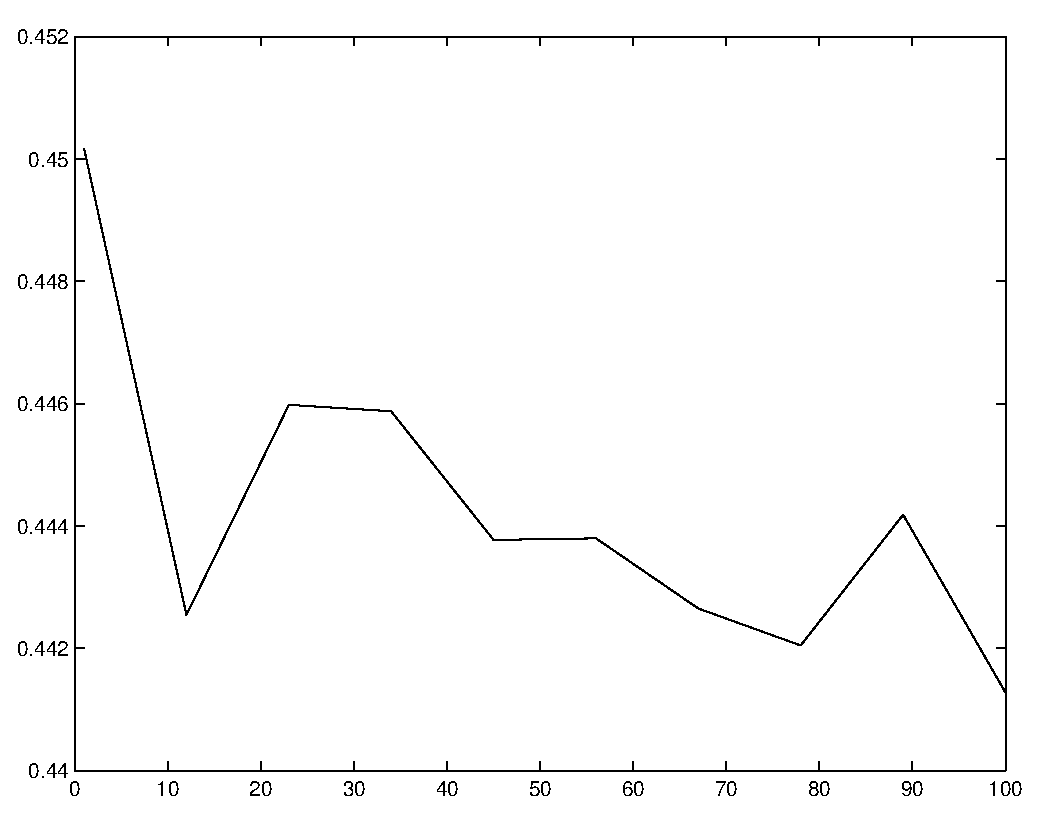
\includegraphics[width=6in]{../../plots/nmf_pseudo/uniform_rdn_rmse_nmf-denorm_median_true.eps} }}
\caption{NMF-Pseudo RMSE-k Plot} \label{fig4}
\end{figure}

\begin{figure}
\centering
\mbox{
\subfigure{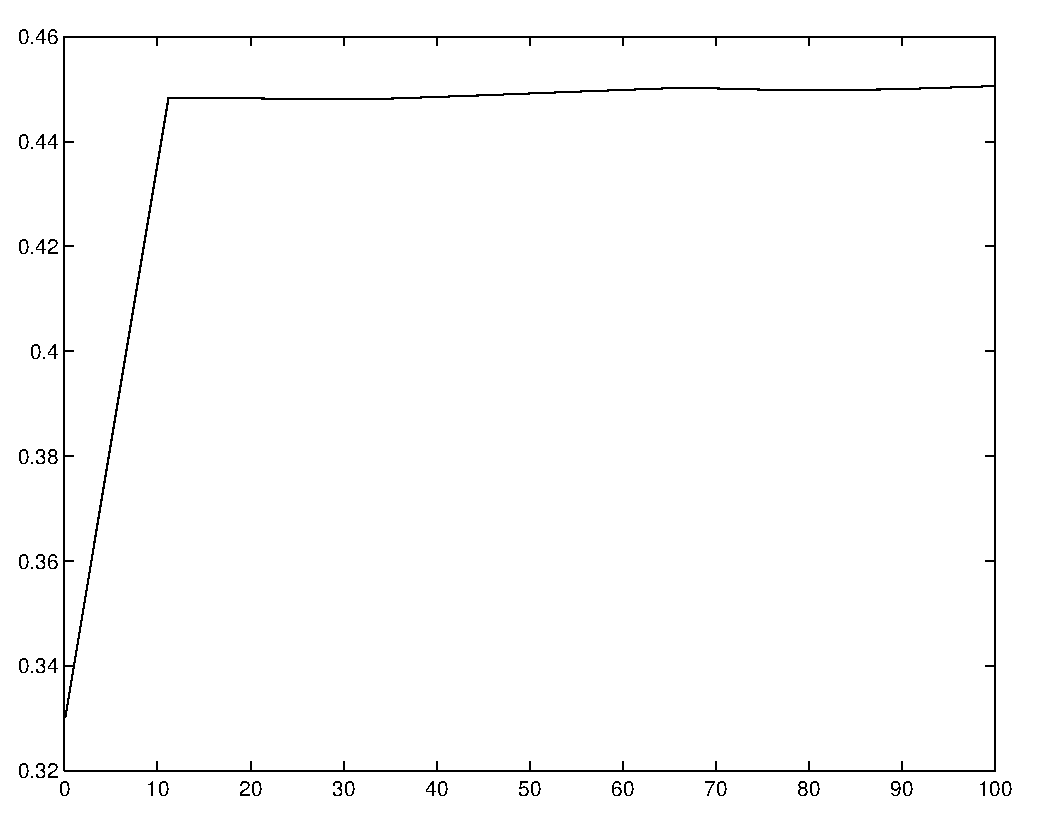
\includegraphics[width=6in]{../../plots/soft_impute_pseudo/soft-impute-denorm_median.eps} }}
\caption{Soft Impute-Pseudo RMSE-$\lambda$ Plot} \label{fig4}
\end{figure}

\end{document}